\documentclass[11pt,letterpaper]{article}

\usepackage[margin=1.03in,headheight=15pt,headsep=18pt,footskip=28pt]{geometry}
\usepackage[T1]{fontenc}
\usepackage[utf8]{inputenc}
\usepackage{lmodern}
\usepackage{microtype}
\usepackage{setspace}
\usepackage{amsmath,amssymb,amsthm,mathtools}
\usepackage{booktabs,array,longtable,tabularx}
\usepackage{enumitem}
\usepackage{fancyhdr}
\usepackage{xcolor}
\usepackage{tikz}
\usetikzlibrary{arrows.meta,positioning,calc,fit,backgrounds}
\usepackage[most]{tcolorbox}
\usepackage{hyperref}
\usepackage{bookmark}
\usepackage{cleveref}

\definecolor{deepblue}{RGB}{28,54,86}
\definecolor{softgray}{RGB}{246,247,249}
\definecolor{linegray}{RGB}{120,125,132}
\hypersetup{
  colorlinks=true,
  linkcolor=deepblue,
  citecolor=deepblue,
  urlcolor=deepblue,
  pdftitle={Shortest Settlement: Optimal Control, Distance Geometry, and Exact One-Dimensional Coordinates for Automated Mathematical Logic Deciders},
  pdfauthor={Brian Tenneson},
  pdfsubject={Optimal conjecture settlement in AMLDs},
  pdfkeywords={automated theorem proving, AMLD, optimal control, Bellman equation, proof search, settlement distance, Abel coordinate}
}

\setstretch{1.08}
\setlength{\parindent}{1.25em}
\setlength{\parskip}{0.18em}
\setlist[itemize]{topsep=3pt,itemsep=2pt,parsep=1pt}
\setlist[enumerate]{topsep=3pt,itemsep=2pt,parsep=1pt}

\pagestyle{fancy}
\fancyhf{}
\fancyhead[L]{\small\textsc{Shortest Settlement}}
\fancyhead[R]{\small Brian Tenneson}
\fancyfoot[C]{\small\thepage}
\renewcommand{\headrulewidth}{0.35pt}
\renewcommand{\footrulewidth}{0pt}

\newtheorem{theorem}{Theorem}[section]
\newtheorem{proposition}[theorem]{Proposition}
\newtheorem{corollary}[theorem]{Corollary}
\newtheorem{lemma}[theorem]{Lemma}
\newtheorem{definition}[theorem]{Definition}
\newtheorem{assumption}[theorem]{Assumption}
\theoremstyle{remark}
\newtheorem{remark}[theorem]{Remark}
\newtheorem{example}[theorem]{Example}
\newtheorem{caution}[theorem]{Caution}

\newtcolorbox{storybox}[1][]{
  colback=softgray,
  colframe=linegray,
  boxrule=0.45pt,
  arc=1.5mm,
  left=2.8mm,right=2.8mm,top=2mm,bottom=2mm,
  title={#1},
  fonttitle=\bfseries
}
\newtcolorbox{statusbox}{
  colback=white,
  colframe=deepblue,
  boxrule=0.65pt,
  arc=1.5mm,
  left=3mm,right=3mm,top=2mm,bottom=2mm
}

\newcommand{\X}{\mathcal X}
\newcommand{\Cset}{\mathcal C}
\newcommand{\Basin}{\mathcal B}
\newcommand{\A}{\mathcal A}
\newcommand{\N}{\mathbb N}
\newcommand{\R}{\mathbb R}
\newcommand{\rstar}{r^{\!*}}
\newcommand{\dset}{D_{\mathrm{set}}}
\newcommand{\rhat}{\widehat r}
\newcommand{\Qstar}{Q^{\!*}}
\newcommand{\argmin}{\operatorname*{arg\,min}}
\newcommand{\argmax}{\operatorname*{arg\,max}}
\newcommand{\dist}{\operatorname{dist}}
\newcommand{\Fix}{\operatorname{Fix}}
\newcommand{\im}{\operatorname{im}}
\newcommand{\Settled}{\operatorname{Settled}}

\title{\bfseries Shortest Settlement\\[0.35em]
\Large Optimal Control, Distance Geometry, and Exact One-Dimensional Coordinates\\
for Automated Mathematical Logic Deciders}
\author{}
\date{}

\begin{document}

\begin{titlepage}
\thispagestyle{empty}
\centering
\vspace*{0.85in}
{\LARGE\bfseries Shortest Settlement\par}
\vspace{0.25in}
{\Large Optimal Control, Distance Geometry, and Exact One-Dimensional Coordinates\par}
{\Large for Automated Mathematical Logic Deciders\par}
\vspace{0.55in}
{\large Version 1.0\par}
\vspace{0.45in}
{\Large Brian Tenneson\par}
\vspace{0.12in}
{\normalsize Bay Path University Alum\par}
{\normalsize M.S. Applied Data Science; M.A. Mathematics\par}
{\normalsize Currently Unaffiliated\par}
\vspace{0.14in}
{\normalsize\href{mailto:btenneson2301@baypath.edu}{btenneson2301@baypath.edu}\par}
{\normalsize\url{https://brian2301.substack.com}\par}
\vfill
{\large August 23, 2026\par}
\vspace{0.25in}
\begin{minipage}{0.82\textwidth}
\small
\centering
A self-contained development of the shortest-settlement control law for verifier-gated conjecture search, including directed settlement distance, Bellman optimality, an exact one-dimensional quotient coordinate, discrete gradient descent, robust approximate compasses, and computational limitations.
\end{minipage}
\vspace{0.45in}
\end{titlepage}

\clearpage
\thispagestyle{empty}
\vspace*{1.15in}
\begin{center}
{\large\bfseries Copyright Notice}
\end{center}
\vspace{0.3in}
\noindent Copyright \textcopyright\ 2026 Brian Tenneson. All rights reserved.

\medskip
\noindent This work may be cited in scholarly discussion with ordinary bibliographic attribution. No license to reproduce, distribute, republish, or create derivative editions is granted except as permitted by law or by written permission of the author.

\vspace{0.35in}
\noindent\textbf{Suggested citation.} Brian Tenneson, \emph{Shortest Settlement: Optimal Control, Distance Geometry, and Exact One-Dimensional Coordinates for Automated Mathematical Logic Deciders}, Version 1.0, August 23, 2026.

\vspace{0.35in}
\noindent\textbf{Contact.} \href{mailto:btenneson2301@baypath.edu}{btenneson2301@baypath.edu}. Essays and project notes: \url{https://brian2301.substack.com}.

\vfill
\begin{statusbox}
\small
\textbf{Status discipline.} This article proves the mathematical claims explicitly labeled theorem, proposition, lemma, or corollary from the hypotheses stated here. It does not claim that an open conjecture has been settled. A theorem characterizing an optimal search policy is not, by itself, an efficient algorithm for computing that policy on arbitrary hard instances. Experimental claims are kept separate from formal results.
\end{statusbox}
\clearpage

\begin{abstract}
A verifier-backed conjecture-settling machine can be modeled as a controlled discrete state system. Its current complete state is a point $x$ in a state space $\X$; admissible actions produce successor states $F_a(x)$; and a verified proof, refutation, independence certificate, or inconsistency certificate places the machine in a terminal settlement set $\Cset$. This article asks a narrow question with broad consequences: what is the mathematically optimal strategy for reaching settlement as quickly as possible?

The answer is exact. On the reachable basin and in the unit-cost model, define $\rstar(x)$ to be the minimum number of further admissible steps required to reach $\Cset$. Then $\rstar$ is exactly the directed distance from $x$ to the settlement set and satisfies the Bellman equation
\[
\rstar(x)=1+\min_{a\in\A(x)}\rstar(F_a(x)).
\]
Consequently, an action is shortest-settlement optimal precisely when it moves to a successor of minimum $\rstar$. This gives a complete feedback characterization of optimal settlement.

The article then makes the geometry precise. The full AMLD state space need not be Euclidean, symmetric, reversible, or contractive. Nevertheless the equivalence relation $x\sim y$ iff $\rstar(x)=\rstar(y)$ produces an exact one-dimensional settlement quotient. The quotient is isometric to an initial segment of the nonnegative integers embedded in $\R$, and every optimal policy is conjugate on this quotient to the elementary shift $k\mapsto k-1$ with $0$ absorbing. Thus optimal settlement has an exact one-dimensional coordinate even though the complete machine state is generally far from one-dimensional. In that coordinate the optimal move is a discrete steepest-descent step, while $h^*=-\rstar$ is an Abel coordinate advancing by $+1$.

Because exact $\rstar$ can be computationally inaccessible, the article proves a sharp robustness result. If an estimated settlement distance $\rhat$ is uniformly accurate to less than $1/2$ on the immediate successor states being compared, greedy descent in $\rhat$ selects a true shortest-settlement action. A more general action-gap theorem covers unequal costs. The final sections distinguish the existence of the optimal coordinate from its computability, show why a total exact settlement-distance oracle would violate undecidability on sufficiently expressive theorem-search classes, and give a concrete blueprint for experimentally learning local settlement geometry without changing verifier semantics.
\end{abstract}

\noindent\textbf{Keywords:} automated theorem proving; automated mathematical logic decider; conjecture settlement; optimal control; Bellman equation; directed distance; proof search; Abel coordinate; value function; verifier-gated search; learned compass.

\medskip
\noindent\textbf{Primary intellectual setting.} This paper isolates and expands the optimal-control thread already present in the broader BANK/SIC/AMLD and settlement-search program, especially the controlled Abel--Bellman theorem and half-step compass guarantee developed in \emph{Verified Settlement Search} \cite{VSS}.

\clearpage
\tableofcontents
\clearpage

\section{Why ask for the shortest settlement?}

The most basic theorem prover asks whether a target can be proved. A broader Automated Mathematical Logic Decider (AMLD) asks for a verified settlement of a target relative to a declared formal environment. Depending on the architecture, settlement may mean a checked proof of the target, a checked proof of its negation, a declared independence metacertificate, or an accepted inconsistency certificate for the base. The common feature is not which channel wins. The common feature is that the machine stops only when a terminal certificate has passed the relevant checker.

That changes the control problem. Once verification is held fixed, the difficult operational question is not merely whether the machine can eventually reach a certificate. It is which legal move should be made \emph{now} if the goal is to arrive at a certificate in the least remaining cost.

\begin{storybox}[A state with four doors]
Imagine that the complete AMLD state is $x$. The BANK already contains some verified lemmas. One proof branch has just failed a unification test. A second branch is open but deep. A reusable lemma is available to prove. The refutation route has barely been explored. The controller has four legal actions $a_1,a_2,a_3,a_4$.

Suppose an omniscient observer knows that after $a_1$ the nearest verified settlement is 19 steps away, after $a_2$ it is 7 steps away, after $a_3$ it is 31 steps away, and after $a_4$ it is 12 steps away. Then the optimal first move is not mysterious: choose $a_2$. The real mathematical question is whether this simple intuition can be stated without smuggling in an undefined notion of ``closeness to proof.''
\end{storybox}

The purpose of this paper is to remove that ambiguity. We will define a directed distance generated by legal AMLD actions, prove that its distance to the settlement set is exactly the minimum-time value function, and derive the optimal feedback law. We will then show that this value supplies an exact one-dimensional quotient geometry of optimal search.

The result is simultaneously stronger and weaker than saying that the complete AMLD state space is Euclidean. It is stronger because the one-dimensional coordinate is exact for the optimization objective. It is weaker because it deliberately forgets all state information except optimal remaining settlement depth. Different BANK contents, proof frontiers, verifier histories, controller states, and resource states may collapse to the same scalar value.

The distinction matters. A representation may be excellent for one control objective without reconstructing the entire state space. In machine-learning language, $\rstar$ is a sufficient scalar target for shortest-settlement control. In dynamic programming, it is a minimum-time value function. In the proof-compass language, it is exact distance-to-settlement. In iteration theory, its negative is an Abel coordinate along optimal trajectories. These are not four metaphors. Under the hypotheses developed below, they are four descriptions of the same object.

\subsection{What is new in this focused treatment}

The broader settlement manuscript already states the controlled Abel--Bellman theorem and the half-step compass guarantee \cite{VSS}. The present article isolates that thread and pushes it farther in five directions.

First, it defines an intrinsic directed control distance $\delta(x,y)$ and proves $\dset(x)=\rstar(x)$ rather than using ``distance'' only informally. Second, it proves that equal-$\rstar$ states form a quotient whose geometry is exactly one-dimensional. Third, it makes the gradient analogy precise at the quotient level and equally precise about where the analogy stops. Fourth, it generalizes the half-step result to an action-gap theorem for unequal costs. Fifth, it proves a computability obstruction showing why the exact coordinate can exist mathematically without yielding a universal effective theorem-decider.

\subsection{Roadmap for the reader}

Sections \ref{sec:model}--\ref{sec:distance} build the controlled AMLD model and its directed geometry. Sections \ref{sec:bellman}--\ref{sec:quotient} prove the central optimality and one-dimensional quotient theorems. Section \ref{sec:gradient} formalizes discrete descent. Section \ref{sec:approx} proves robustness of approximate compasses. Section \ref{sec:weighted} handles unequal costs. Sections \ref{sec:channels}--\ref{sec:bank} return the theory to P/R/I/C settlement and verified BANK state. Section \ref{sec:limits} proves the computability limitation. The last sections give an implementation blueprint and an experimental design that can test learned settlement geometry without weakening proof verification.

\section{The controlled AMLD state model}\label{sec:model}

\subsection{Complete state}

A control theorem is only as meaningful as its state variable. If the controller is told that the current state is merely ``the target formula,'' then two moments of search with radically different BANK contents and proof frontiers become indistinguishable. A Markov control model therefore uses a \emph{complete} operational state.

\begin{definition}[Complete AMLD state space]
Let $\X$ be the set of admissible complete states of a fixed AMLD environment. A state $x\in\X$ contains every variable required to determine the next verified transition once a control action has been selected. Schematically one may write
\[
x=(B,FB,H,\mathrm{Ref},\mathrm{Ctrl},R,q,\ldots),
\]
where $B$ is the verified BANK, $FB$ a counterfactual or future-search structure, $H$ a history record, $\mathrm{Ref}$ checked reflective state, $\mathrm{Ctrl}$ controller state, $R$ resource state, and $q$ phase or scheduler information. The exact coordinates are implementation-dependent.
\end{definition}

The definition is intentionally abstract. It does not require that every implementation literally use these fields. It requires only enough state to make the declared transition law well-defined. This is the same Markov-completeness requirement used in the controlled-system formulation of the larger AMLD program \cite{VSS,DATA3}.

\begin{definition}[Admissible actions and transitions]
For each $x\in\X$, let $\A(x)$ be the set of admissible control actions. Each $a\in\A(x)$ determines a successor
\[
F_a(x)\in\X.
\]
An action may allocate a search quantum to a P/R/I/C role, expand a proof branch, test a candidate assertion, prove a reusable lemma, perform a verifier-neutral representation change, or execute any other declared atomic control operation.
\end{definition}

We treat $F_a$ as deterministic after all randomness needed for the next update is included in the complete state. Equivalently, a random seed or random-generator state can be part of $x$. Nothing fundamental depends on this bookkeeping choice; it merely avoids mixing stochastic-control notation into the main theorem.

\subsection{Settlement states}

\begin{definition}[Terminal settlement set]
Let $\Cset\subseteq\X$ be the set of states containing an accepted terminal settlement certificate and terminal status. A state in $\Cset$ is called a \emph{settlement state}.
\end{definition}

For the standard four-channel AMLD interpretation, $\Cset$ may be decomposed as
\[
\Cset=\Cset_P\cup\Cset_R\cup\Cset_I\cup\Cset_C,
\]
corresponding to proof, refutation, independence, and inconsistency channels. This union is operational: whichever declared certificate is accepted first terminates the search according to the architecture's priority rules.

\begin{assumption}[Terminal freezing]\label{ass:freeze}
For every $s\in\Cset$, the AMLD makes no further mathematical search progress. Formally, either $\A(s)=\varnothing$, or every declared post-terminal action leaves the state fixed: $F_a(s)=s$.
\end{assumption}

Terminal freezing converts settlement into fixed-point geometry. Under an autonomous terminalized update $T$, one may have $\Fix(T)=\Cset$ when nonterminal states are forced to change an appropriate counter, as developed in the prior settlement manuscript \cite{VSS}. The present paper needs less: it needs only that reaching $\Cset$ ends the optimization problem.

\subsection{Reachability and the settlement basin}

\begin{definition}[Finite legal trajectory]
A finite legal trajectory from $x$ is a sequence
\[
x_0=x,x_1,\ldots,x_m
\]
with actions $a_0,\ldots,a_{m-1}$ such that $a_k\in\A(x_k)$ and
\[
x_{k+1}=F_{a_k}(x_k)
\]
for $0\le k<m$.
\end{definition}

\begin{definition}[Reachable settlement basin]
The reachable settlement basin is
\[
\Basin=\{x\in\X:\text{some finite legal trajectory from $x$ reaches $\Cset$}\}.
\]
\end{definition}

The restriction to $\Basin$ is essential. A fixed-point theorem says what a settlement state looks like; it does not imply that every starting state reaches one. An AMLD can time out, enter a nonsettling region under a poor policy, or face a target for which the declared certificate family is not effectively reachable. We therefore prove shortest-settlement statements on states from which settlement is actually reachable.

\begin{storybox}[A fixed point is not a promise]
A train station can be perfectly well defined even if no track from the current town reaches it. In the same way, identifying $\Cset$ as the absorbing fixed-point set does not show that the current AMLD state lies in its basin. The optimization problem begins only after reachability is separated from the definition of the destination.
\end{storybox}

\section{The intrinsic directed geometry of legal search}\label{sec:distance}

The first temptation is to place $\X$ inside a Euclidean vector space and write an ordinary metric $d(x,s)$. That can be useful as a learned representation, but it is not the intrinsic geometry of proof search. Proof-search transitions are directed. A verified lemma may be deposited and never ``undeposited.'' A substitution may constrain future branches in a way that cannot be reversed by any legal action. Resource counters usually increase. Histories accumulate.

The natural primitive is therefore a directed path distance generated by legal actions.

\subsection{Unit-cost directed distance}

We begin with the unit-cost model in which every atomic control step costs one.

\begin{definition}[Directed unit-cost distance]
For $x,y\in\X$, define
\[
\delta(x,y)=\min\{m\in\N_0:\text{there is a legal trajectory of length $m$ from $x$ to $y$}\},
\]
when such a trajectory exists, and set $\delta(x,y)=+\infty$ otherwise.
\end{definition}

Because the set of attainable finite path lengths is a nonempty subset of $\N_0$ whenever $y$ is reachable from $x$, the minimum exists.

\begin{proposition}[Directed graph-distance properties]\label{prop:directedmetric}
For all $x,y,z\in\X$:
\begin{enumerate}[label=(\roman*)]
\item $\delta(x,x)=0$;
\item if $\delta(x,y)=0$, then $x=y$;
\item $\delta(x,z)\le \delta(x,y)+\delta(y,z)$, with the usual extended-real convention;
\item symmetry need not hold: in general $\delta(x,y)\ne\delta(y,x)$.
\end{enumerate}
\end{proposition}

\begin{proof}
The empty trajectory gives (i). A length-zero trajectory has only its initial state, giving (ii). If finite trajectories of lengths $m$ and $n$ connect $x$ to $y$ and $y$ to $z$, concatenation gives a trajectory of length $m+n$ from $x$ to $z$; minimizing yields (iii). For (iv), take two states with one legal transition $x\to y$ and no legal path from $y$ to $x$. Then $\delta(x,y)=1$ and $\delta(y,x)=+\infty$.
\end{proof}

Thus $\delta$ is an extended directed graph distance, not an ordinary metric. This is not a defect. It records irreversibility that a symmetric Euclidean metric would erase.

\subsection{Distance to the settlement set}

\begin{definition}[Settlement distance]
For $x\in\Basin$, define
\[
\dset(x)=\min_{s\in\Cset}\delta(x,s).
\]
Equivalently, $\dset(x)$ is the minimum length of any finite legal trajectory beginning at $x$ and ending in a settlement state.
\end{definition}

The minimum exists because $x\in\Basin$ and attainable path lengths to $\Cset$ form a nonempty subset of $\N_0$.

\begin{proposition}[Zero set]\label{prop:zeroset}
For $x\in\Basin$,
\[
\dset(x)=0\quad\Longleftrightarrow\quad x\in\Cset.
\]
\end{proposition}

\begin{proof}
If $x\in\Cset$, then $\delta(x,x)=0$, so $\dset(x)=0$. Conversely, if $\dset(x)=0$, some $s\in\Cset$ satisfies $\delta(x,s)=0$. By Proposition \ref{prop:directedmetric}(ii), $x=s$, hence $x\in\Cset$.
\end{proof}

This corrects a common but important notational slip. If one fixes a settlement point $S$ and writes $\inf_{x\in\X}d(x,S)$, the answer is trivially zero because $x=S$ is allowed. The meaningful control quantity fixes the \emph{current} state $x$ and minimizes over reachable settlement states:
\[
\inf_{s\in\Cset}\delta(x,s).
\]
In the unit-cost setting the infimum is a minimum and equals $\dset(x)$.

\begin{figure}[ht]
\centering
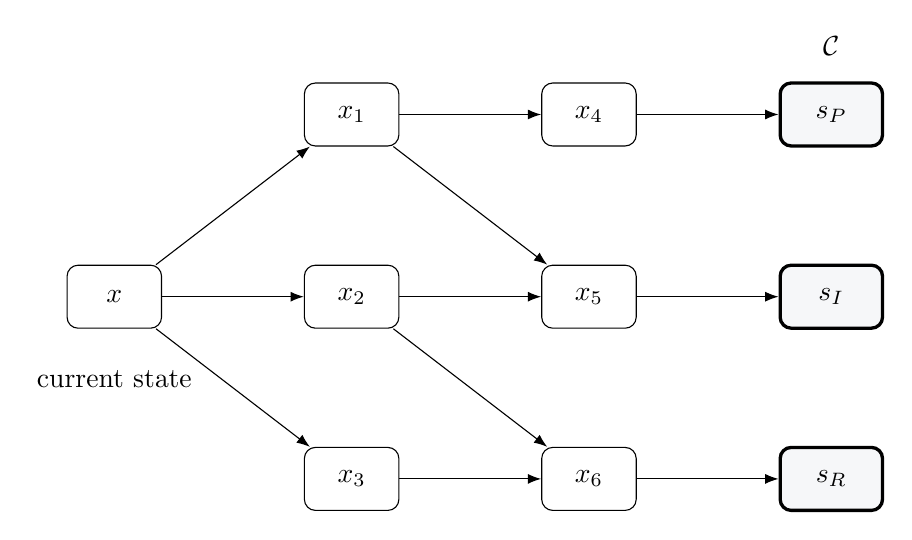
\begin{tikzpicture}[>=Latex, node distance=15mm and 18mm,
 state/.style={draw,rounded corners,minimum width=12mm,minimum height=8mm,fill=white},
 term/.style={draw,rounded corners,minimum width=13mm,minimum height=8mm,fill=softgray,very thick}]
\node[state] (x) {$x$};
\node[state, above right=of x] (a) {$x_1$};
\node[state, right=of x] (b) {$x_2$};
\node[state, below right=of x] (c) {$x_3$};
\node[state, right=of a] (a2) {$x_4$};
\node[state, right=of b] (b2) {$x_5$};
\node[state, right=of c] (c2) {$x_6$};
\node[term, right=of a2] (sp) {$s_P$};
\node[term, right=of b2] (si) {$s_I$};
\node[term, right=of c2] (sr) {$s_R$};
\draw[->] (x)--(a); \draw[->] (x)--(b); \draw[->] (x)--(c);
\draw[->] (a)--(a2); \draw[->] (a2)--(sp);
\draw[->] (b)--(b2); \draw[->] (b2)--(si);
\draw[->] (c)--(c2); \draw[->] (c2)--(sr);
\draw[->,bend left=20] (a)--(b2);
\draw[->,bend right=18] (b)--(c2);
\node[below=4mm of x,align=center] {current\ state};
\node[above=2mm of sp] {$\Cset$};
\end{tikzpicture}
\caption{Settlement is distance to a \emph{set} of terminal states through legal directed transitions. Different certificate channels can terminate in different complete states.}
\label{fig:directed}
\end{figure}

\section{Optimal remaining settlement time}\label{sec:bellman}

We now define the same quantity in the language of policies. The equivalence with directed settlement distance is the first central theorem.

\begin{definition}[Policy and settlement time]
A deterministic feedback policy $\pi$ assigns to each nonterminal state in its domain an admissible action $\pi(x)\in\A(x)$. Starting from $x_0=x$, the policy trajectory satisfies
\[
x_{n+1}=F_{\pi(x_n)}(x_n)
\]
until a settlement state is reached. Let $\tau_\pi(x)$ be the first $n\ge0$ for which $x_n\in\Cset$, with $\tau_\pi(x)=+\infty$ if no such $n$ occurs.
\end{definition}

\begin{definition}[Optimal remaining settlement time]
For $x\in\Basin$, define
\[
\rstar(x)=\min_{\pi}\tau_\pi(x),
\]
where the minimum ranges over policies that settle from $x$.
\end{definition}

One could instead minimize over finite action sequences. For deterministic dynamics the definitions agree. The policy formulation matters because our eventual strategy will be a feedback rule defined from the current complete state.

\begin{theorem}[Settlement distance equals optimal remaining time]\label{thm:distanceequals}
For every $x\in\Basin$,
\[
\boxed{\dset(x)=\rstar(x).}
\]
\end{theorem}

\begin{proof}
Every policy trajectory that settles from $x$ is a legal trajectory from $x$ to some $s\in\Cset$. Hence its settlement time is at least $\dset(x)$, so $\rstar(x)\ge\dset(x)$.

Conversely, choose a legal trajectory of minimum length $\dset(x)$ from $x$ to $\Cset$. Define a policy along the finitely many nonterminal states on that trajectory to select the corresponding next action; define it arbitrarily elsewhere. This policy settles from $x$ in exactly $\dset(x)$ steps. Thus $\rstar(x)\le\dset(x)$. The two inequalities give equality.
\end{proof}

The theorem makes ``distance to settlement'' literal. In the unit-cost model, the value function is not merely correlated with shortest path length. It \emph{is} shortest path length in the directed control graph.

\subsection{The Bellman decomposition}

Let $x\in\Basin\setminus\Cset$. Any successful trajectory must take a first action and then continue from the successor. This obvious decomposition is exactly the Bellman principle of optimality \cite{Bellman}.

\begin{theorem}[Shortest-settlement Bellman theorem]\label{thm:bellman}
For every nonterminal $x\in\Basin$,
\[
\boxed{\rstar(x)=1+\min_{a\in\A(x)\,:\,F_a(x)\in\Basin}\rstar(F_a(x)).}
\]
Moreover, an admissible action $a$ is the first action of a shortest settlement trajectory from $x$ if and only if
\[
\rstar(F_a(x))=\rstar(x)-1.
\]
\end{theorem}

\begin{proof}
Let $m=\rstar(x)$. A shortest settlement trajectory from $x$ has length $m\ge1$ and begins with some action $a^*$. Its successor $y=F_{a^*}(x)$ settles in exactly $m-1$ further steps; otherwise the original trajectory would not be shortest. Thus $\rstar(y)=m-1$, proving
\[
1+\min_a\rstar(F_a(x))\le m.
\]
For any admissible first action $a$ with successor in $\Basin$, every settlement trajectory from $F_a(x)$ requires at least $\rstar(F_a(x))$ further steps, so every settlement trajectory beginning with $a$ has length at least $1+\rstar(F_a(x))$. Minimizing over first actions gives
\[
m\le1+\min_a\rstar(F_a(x)).
\]
Hence equality holds. The final equivalence follows immediately: a first action is shortest-settlement exactly when it attains the minimum, which is equivalent to $\rstar(F_a(x))=m-1$.
\end{proof}

\begin{definition}[Optimal-action correspondence]
For $x\in\Basin\setminus\Cset$, define
\[
\A^*(x)=\argmin_{a\in\A(x),\,F_a(x)\in\Basin}\rstar(F_a(x)).
\]
By Theorem \ref{thm:bellman}, $\A^*(x)$ is nonempty and
\[
a\in\A^*(x)\quad\Longleftrightarrow\quad \rstar(F_a(x))=\rstar(x)-1.
\]
\end{definition}

We can therefore state the optimal strategy in one line:
\[
\boxed{\pi^*(x)\in\A^*(x).}
\]
If the implementation has a fixed total ordering of admissible actions, choose the least member of $\A^*(x)$ to obtain a canonical deterministic selector. No ambiguity remains at the level of optimality: ties correspond to genuinely equally short first moves.

\begin{corollary}[Exact shortest-settlement feedback]\label{cor:policy}
Let $\pi^*$ select an action in $\A^*(x)$ at every nonterminal state $x\in\Basin$. Then for every $x_0\in\Basin$, the trajectory under $\pi^*$ reaches $\Cset$ after exactly $\rstar(x_0)$ steps.
\end{corollary}

\begin{proof}
If $x_n\notin\Cset$, Theorem \ref{thm:bellman} gives
\[
\rstar(x_{n+1})=\rstar(x_n)-1.
\]
Induction yields $\rstar(x_n)=\rstar(x_0)-n$ until the value reaches zero. By Proposition \ref{prop:zeroset} and Theorem \ref{thm:distanceequals}, value zero is equivalent to settlement. Therefore settlement occurs exactly at $n=\rstar(x_0)$.
\end{proof}

\subsection{The result in plain language}

The theorem does not say ``always choose the syntactically simplest lemma,'' ``always expand the shallowest proof branch,'' or ``always prefer the prover channel.'' It says something both more general and more demanding:

\begin{center}
\emph{At each state, choose a legal successor with the smallest true optimal remaining settlement distance.}
\end{center}

Every concrete heuristic is good only insofar as it approximates that ordering under the cost model one actually cares about.

\begin{storybox}[The seven-step door]
Return to the four-door state from the opening. If the successor distances are 19, 7, 31, and 12, the Bellman theorem says that the current state has value $1+7=8$. Choosing the seven-step successor is not merely plausible; it is the unique shortest-settlement choice if the other three values are strictly larger. After the move, the same theorem is applied again. The policy is local in execution but globally optimal because the value already summarizes the best possible future continuation.
\end{storybox}

\section{Geodesics of verified settlement}\label{sec:geodesics}

The word \emph{geodesic} usually evokes smooth manifolds, but at its most basic it means a shortest path with respect to a distance. In a directed discrete control graph, the corresponding object is immediate.

\begin{definition}[Settlement geodesic]
A legal trajectory
\[
x_0,x_1,\ldots,x_m
\]
with $x_m\in\Cset$ is a settlement geodesic from $x_0$ if $m=\dset(x_0)=\rstar(x_0)$.
\end{definition}

\begin{proposition}[Characterization of settlement geodesics]\label{prop:geodesic}
A settling trajectory $x_0,\ldots,x_m$ is a settlement geodesic if and only if
\[
\rstar(x_{k+1})=\rstar(x_k)-1
\]
for every $0\le k<m$.
\end{proposition}

\begin{proof}
If the displayed equality holds at every step, then $\rstar(x_k)=\rstar(x_0)-k$. Since $x_m\in\Cset$, $\rstar(x_m)=0$, hence $m=\rstar(x_0)$ and the path is shortest.

Conversely, every suffix of a shortest path is shortest between its starting point and $\Cset$; otherwise replacing the suffix by a shorter settlement path would shorten the original trajectory. Therefore the suffix beginning at $x_k$ has length $m-k=\rstar(x_k)$, so $\rstar(x_{k+1})=m-k-1=\rstar(x_k)-1$.
\end{proof}

\begin{definition}[Settlement projection]
For $x\in\Basin$, define the set of nearest terminal states
\[
\Pi_{\Cset}(x)=\{s\in\Cset:\delta(x,s)=\dset(x)\}.
\]
\end{definition}

The projection can be set-valued. Two distinct certificates, or even two distinct settlement channels, may lie at equal minimum distance. This is another reason not to force the complete terminal set into a single Euclidean point too early. The optimization objective cares about the nearest terminal class; provenance may care which terminal state is reached.

\begin{proposition}[Distance to a union of settlement channels]\label{prop:union}
Suppose $\Cset=\bigcup_{j\in J}\Cset_j$. Define
\[
D_j(x)=\min_{s\in\Cset_j}\delta(x,s),
\]
with $D_j(x)=+\infty$ when $\Cset_j$ is unreachable. Then
\[
\dset(x)=\min_{j\in J}D_j(x).
\]
\end{proposition}

\begin{proof}
Both sides are the minimum of $\delta(x,s)$ over the same union of terminal states, with the right side grouping the minimization by channel.
\end{proof}

For P/R/I/C settlement this says the nearest verified outcome controls the unit-cost minimum-time objective. If the architecture assigns different priorities or costs to different terminal outcomes, the objective must be modified accordingly; Section \ref{sec:weighted} handles that generalization.

\section{The exact one-dimensional settlement quotient}\label{sec:quotient}

We can now answer the geometric question that motivated this article. Does the optimal settlement problem admit a low-dimensional representation that preserves both distance-to-settlement and the direction of optimal motion?

Yes. In the unit-cost model it admits an exact one-dimensional representation. The important qualification is that this representation is naturally a \emph{quotient} of the complete state space, not an isomorphism of the complete AMLD state with a Euclidean vector space.

\subsection{Collapsing states of equal optimal depth}

\begin{definition}[Equal-depth equivalence relation]
For $x,y\in\Basin$, write
\[
x\sim y\quad\Longleftrightarrow\quad \rstar(x)=\rstar(y).
\]
Let
\[
\Basin_{\!*}=\Basin/\!\sim
\]
be the quotient set, and write $[x]$ for the equivalence class of $x$.
\end{definition}

The quotient deliberately forgets how a state obtained its current BANK, which proof branch is open, what the verifier history looks like, and every other feature not determined by optimal remaining depth. Two states are equivalent exactly when the shortest possible number of remaining steps is the same.

\begin{definition}[Settlement coordinate]
Define
\[
\Phi:\Basin\to\N_0,\qquad \Phi(x)=\rstar(x).
\]
The induced map on the quotient is
\[
\overline\Phi:\Basin_{\!*}\to\N_0,\qquad \overline\Phi([x])=\rstar(x).
\]
\end{definition}

The quotient map is well-defined by construction.

\begin{lemma}[The image is an initial segment]\label{lem:initialsegment}
The set $\im(\Phi)\subseteq\N_0$ is downward closed. Hence it is either
\[
\{0,1,\ldots,K\}
\]
for some $K\in\N_0$, or all of $\N_0$.
\end{lemma}

\begin{proof}
Let $k\in\im(\Phi)$. Then there is $x\in\Basin$ with $\rstar(x)=k$. If $k=0$, there is nothing to prove. If $k>0$, Corollary \ref{cor:policy} gives an optimal trajectory $x=x_0,x_1,\ldots,x_k$ with
\[
\rstar(x_j)=k-j.
\]
Thus every integer from $0$ through $k$ lies in the image. Therefore the image is downward closed in $\N_0$, which has exactly the stated forms.
\end{proof}

\begin{theorem}[Exact one-dimensional settlement quotient]\label{thm:quotient}
The induced coordinate
\[
\overline\Phi:\Basin_{\!*}\longrightarrow \im(\Phi)
\]
is a bijection. Define
\[
d_{\!*}([x],[y])=|\rstar(x)-\rstar(y)|.
\]
Then $d_{\!*}$ is a metric on $\Basin_{\!*}$ and $\overline\Phi$ is an isometry from $(\Basin_{\!*},d_{\!*})$ onto the initial segment $\im(\Phi)\subseteq\R$ with its ordinary Euclidean metric.

Moreover, the entire settlement set $\Cset$ is one quotient class, denoted $[\Cset]$, and
\[
\boxed{d_{\!*}([x],[\Cset])=\rstar(x)=\dset(x).}
\]
\end{theorem}

\begin{proof}
If $[x]=[y]$, then $\rstar(x)=\rstar(y)$, so $\overline\Phi$ is well-defined. It is injective because equal values imply $x\sim y$ and therefore $[x]=[y]$. It is surjective onto $\im(\Phi)$ by definition of the image.

Since $\overline\Phi$ is a bijection and
\[
d_{\!*}(u,v)=|\overline\Phi(u)-\overline\Phi(v)|,
\]
the metric axioms follow from the Euclidean metric on $\R$, and $\overline\Phi$ is an isometry.

By Proposition \ref{prop:zeroset} and Theorem \ref{thm:distanceequals}, $\rstar(x)=0$ exactly for $x\in\Cset$. Thus all terminal states lie in the same quotient class and no nonterminal state lies in that class. Finally,
\[
d_{\!*}([x],[\Cset])=|\rstar(x)-0|=\rstar(x)=\dset(x).
\]
\end{proof}

This theorem gives the exact affirmative answer. There exists a one-dimensional Euclidean settlement geometry in which distance to the terminal class is exactly true optimal remaining settlement distance. It is not an approximation and does not require learning.

What it does require is quotienting. The full state $x$ and the scalar $\rstar(x)$ are not the same mathematical object.

\begin{storybox}[Two machines, both six steps away]
One AMLD state may contain twenty verified lemmas and a narrow proof frontier. Another may contain only five lemmas but a refutation branch that happens to be close to completion. Their complete states can be utterly different. If both have $\rstar=6$, the settlement quotient identifies them.

That identification would be disastrous if one were trying to reconstruct the BANK or explain the search history. It is perfect if the only question is ``how many optimal steps remain?'' A quotient is allowed to forget information precisely because it is designed for a specified purpose.
\end{storybox}

\subsection{Optimal dynamics become the shift}

Fix any optimal selector $\pi^*$ and define the terminalized optimal map
\[
T^*(x)=
\begin{cases}
F_{\pi^*(x)}(x),&x\notin\Cset,\\
x,&x\in\Cset.
\end{cases}
\]
Define the one-dimensional shift
\[
S(k)=\max(k-1,0),\qquad k\in\im(\Phi).
\]

\begin{theorem}[Semiconjugacy and quotient conjugacy]\label{thm:conjugacy}
For every $x\in\Basin$,
\[
\boxed{\Phi(T^*(x))=S(\Phi(x)).}
\]
Thus $\Phi$ semiconjugates optimal AMLD dynamics to the one-dimensional shift.

Furthermore, $T^*$ induces a well-defined map $\overline T^*$ on $\Basin_{\!*}$ by
\[
\overline T^*([x])=[T^*(x)],
\]
and
\[
\boxed{\overline\Phi\circ\overline T^*=S\circ\overline\Phi.}
\]
Since $\overline\Phi$ is bijective, the quotient dynamics are conjugate to the shift $S$.
\end{theorem}

\begin{proof}
If $x\in\Cset$, then $T^*(x)=x$ and $\Phi(x)=0$, so both sides equal $0$. If $x\notin\Cset$, optimality gives
\[
\rstar(T^*(x))=\rstar(x)-1,
\]
which is exactly $\Phi(T^*(x))=S(\Phi(x))$.

To show that $\overline T^*$ is well-defined, suppose $x\sim y$. Then $\rstar(x)=\rstar(y)=k$. If $k=0$, both are terminal and their images have value $0$. If $k>0$, optimality gives
\[
\rstar(T^*(x))=k-1=\rstar(T^*(y)),
\]
so $T^*(x)\sim T^*(y)$. Hence the quotient map is well-defined. The conjugacy identity follows from the first identity and the definition of $\overline\Phi$.
\end{proof}

\begin{figure}[ht]
\centering
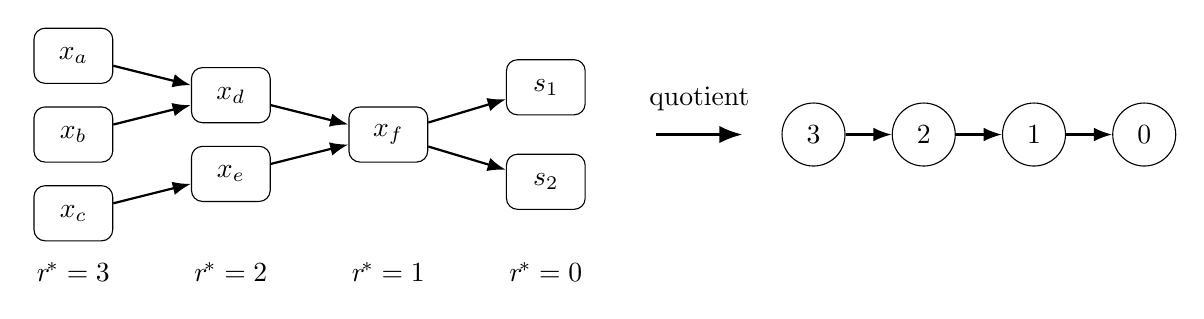
\begin{tikzpicture}[>=Latex,
 state/.style={draw,rounded corners,minimum width=10mm,minimum height=7mm},
 lvl/.style={draw,circle,minimum size=8mm}]
\node[state] (a) at (0,2.0) {$x_a$};
\node[state] (b) at (0,1.0) {$x_b$};
\node[state] (c) at (0,0.0) {$x_c$};
\node[state] (d) at (2.0,1.5) {$x_d$};
\node[state] (e) at (2.0,0.5) {$x_e$};
\node[state] (f) at (4.0,1.0) {$x_f$};
\node[state] (s1) at (6.0,1.6) {$s_1$};
\node[state] (s2) at (6.0,0.4) {$s_2$};
\draw[->,thick] (a)--(d); \draw[->,thick] (b)--(d); \draw[->,thick] (c)--(e);
\draw[->,thick] (d)--(f); \draw[->,thick] (e)--(f);
\draw[->,thick] (f)--(s1); \draw[->,thick] (f)--(s2);
\node at (0,-0.75) {$\rstar=3$};
\node at (2,-0.75) {$\rstar=2$};
\node at (4,-0.75) {$\rstar=1$};
\node at (6,-0.75) {$\rstar=0$};

\draw[->,very thick] (7.4,1.0)--(8.5,1.0);
\node[align=center] at (7.95,1.45) {quotient};

\node[lvl] (l3) at (9.4,1.0) {3};
\node[lvl] (l2) at (10.8,1.0) {2};
\node[lvl] (l1) at (12.2,1.0) {1};
\node[lvl] (l0) at (13.6,1.0) {0};
\draw[->,thick] (l3)--(l2); \draw[->,thick] (l2)--(l1); \draw[->,thick] (l1)--(l0);
\end{tikzpicture}
\caption{Many complete states can occupy the same optimal settlement depth. Quotienting by equal $\rstar$ collapses the optimal dynamics to the exact one-dimensional shift $3\to2\to1\to0$.}
\label{fig:quotient}
\end{figure}

\subsection{Why this is not $\X\cong\R^n$}

The quotient theorem should not be overstated. It does not say that the complete state space is a Euclidean vector space, nor that every pairwise directed control distance is preserved by $\Phi$.

\begin{proposition}[Irreversibility obstructs an isometric Euclidean model of the directed distance]\label{prop:noeuclid}
Suppose there exist $x,y\in\X$ with $\delta(x,y)<\infty$ and $\delta(y,x)=+\infty$. Then no map $E:\X\to\R^n$ can satisfy
\[
\|E(x)-E(y)\|=\delta(x,y)
\]
for all ordered pairs $x,y$.
\end{proposition}

\begin{proof}
If such $E$ existed, symmetry of Euclidean distance would give
\[
\delta(x,y)=\|E(x)-E(y)\|=\|E(y)-E(x)\|=\delta(y,x),
\]
contradicting the assumed finite/infinite asymmetry.
\end{proof}

So the correct structural statement is
\[
\boxed{\text{complete state space: generally non-Euclidean and directed;}}
\]
while
\[
\boxed{\text{optimal settlement quotient: exactly one-dimensional Euclidean.}}
\]

That distinction is central to the paper.

\section{Discrete gradient descent toward settlement}\label{sec:gradient}

The original geometric intuition was to attach to the current AMLD state $x$ both a distance to the nearest settlement and a direction arrow pointing downhill, perhaps analogous to a negative gradient. We can now make that statement exact on the settlement quotient.

\subsection{The scalar potential}

Identify $\Basin_{\!*}$ with $\im(\Phi)\subseteq\R_{\ge0}$ through $\overline\Phi$. Define the settlement potential
\[
V(z)=z,
\qquad z\ge0.
\]
For $z>0$,
\[
\nabla V(z)=1,
\qquad -\nabla V(z)=-1.
\]
An optimal AMLD move changes the settlement coordinate by exactly
\[
\Phi(T^*x)-\Phi(x)=-1
\]
for nonterminal $x$. Thus the optimal discrete step has exactly the same direction and magnitude as the negative gradient of $V$ in the one-dimensional quotient.

\begin{theorem}[Exact discrete gradient representation]\label{thm:gradient}
Let $x\in\Basin\setminus\Cset$ and let $a\in\A(x)$ have successor $y=F_a(x)$. Define the settlement-coordinate increment
\[
\Delta_a\Phi(x)=\Phi(y)-\Phi(x).
\]
Then
\[
\min_{a\in\A(x),\,F_a(x)\in\Basin}\Delta_a\Phi(x)=-1,
\]
and
\[
a\in\A^*(x)\quad\Longleftrightarrow\quad \Delta_a\Phi(x)=-1.
\]
Under the quotient identification $z=\Phi(x)$, this optimal increment equals $-\nabla V(z)$ for $V(z)=z$ and $z>0$.
\end{theorem}

\begin{proof}
Theorem \ref{thm:bellman} gives $\rstar(F_a(x))\ge\rstar(x)-1$ for every successor in the settlement basin, with equality exactly for optimal actions. Subtracting $\rstar(x)$ gives the first two statements. Since $V'(z)=1$ for $z>0$, the optimal increment $-1$ equals $-\nabla V(z)$.
\end{proof}

\begin{definition}[Optimal settlement arrow]
The intrinsic discrete settlement arrow at $x$ is the set-valued correspondence
\[
\operatorname{Arrow}(x)=\A^*(x).
\]
If a vector representation of admissible actions is available, one may instead represent each $a\in\A(x)$ by a displacement vector and mark those vectors corresponding to $\A^*(x)$.
\end{definition}

The arrow is naturally set-valued because multiple equally short actions can exist. A single deterministic arrow requires a tie-break rule, not new mathematics.

\begin{storybox}[The hiker who can use only trails]
A hiker on a smooth hillside can, in principle, walk directly in the direction $-\nabla V$. An AMLD cannot. It is allowed to perform only declared inference, search, memory, and control actions. The right analogy is therefore a hiker standing at a trail junction: the scalar landscape says which way is downhill, but motion is restricted to the available trails.

In the exact settlement quotient something stronger happens. At every reachable nonterminal state, at least one legal trail realizes the full one-unit downhill step. That fact is not supplied by differential geometry; it is supplied by the definition of $\rstar$ and the existence of a shortest legal trajectory.
\end{storybox}

\subsection{The Abel coordinate}

Define
\[
h^*(x)=-\rstar(x).
\]
Then an optimal move satisfies
\[
h^*(T^*x)=h^*(x)+1
\]
before settlement. This is the additive Abel equation along the optimal dynamics.

\begin{corollary}[Optimal Abel coordinate]\label{cor:abel}
For nonterminal $x\in\Basin$,
\[
\boxed{h^*(T^*x)=h^*(x)+1.}
\]
Equivalently,
\[
\max_{a\in\A(x)}h^*(F_a(x))=h^*(x)+1.
\]
\end{corollary}

\begin{proof}
Since $h^*=-\rstar$, Theorem \ref{thm:bellman} gives
\[
\max_a h^*(F_a(x))=-\min_a\rstar(F_a(x))=-(\rstar(x)-1)=h^*(x)+1.
\]
An optimal selector attains the maximum.
\end{proof}

The equation cannot hold at a fixed terminal point with a finite Abel coordinate, because $T^*s=s$ would force $h^*(s)=h^*(s)+1$. Thus the translation coordinate belongs to the pre-settlement basin and terminates at the absorbing boundary, exactly as in the earlier settlement analysis \cite{VSS}.

\section{Approximate settlement compasses}\label{sec:approx}

The exact coordinate solves the control problem conceptually but may be expensive to compute. On a hard theorem search, asking for $\rstar(x)$ can be nearly as difficult as asking the search itself to find the shortest proof route. The practical controller therefore needs an estimate.

Let
\[
\rhat:\Basin\to\R
\]
be an estimated remaining settlement distance. The simplest greedy controller chooses
\[
\widehat\pi(x)\in\argmin_{a\in\A(x)}\rhat(F_a(x)).
\]
The question is how accurate $\rhat$ must be in order to recover the true optimal action.

\subsection{Why one half appears}

In the unit-cost model, $\rstar$ is integer-valued. At a state of depth $k>0$, every optimal successor has depth $k-1$. Every nonoptimal successor in the settlement basin has depth at least $k$. Therefore the true gap between an optimal and nonoptimal successor is at least one integer unit.

That spacing makes the threshold $1/2$ exact and natural.

\begin{theorem}[Half-step compass theorem]\label{thm:halfstep}
Let $x\in\Basin\setminus\Cset$. Suppose that for every candidate successor $y=F_a(x)\in\Basin$,
\[
|\rhat(y)-\rstar(y)|<\frac12.
\]
Then every minimizer of $\rhat(F_a(x))$ is a true shortest-settlement action:
\[
\argmin_a \rhat(F_a(x))\subseteq \A^*(x).
\]
If the same error condition holds at every state encountered by the greedy $\rhat$-controller, then starting from $x_0$ it reaches settlement in exactly $\rstar(x_0)$ steps.
\end{theorem}

\begin{proof}
Let $k=\rstar(x)$. For any optimal successor $y^*$,
\[
\rstar(y^*)=k-1,
\]
so
\[
\rhat(y^*)<k-\frac12.
\]
For any nonoptimal successor $z$, integer-valuedness and Theorem \ref{thm:bellman} imply $\rstar(z)\ge k$, hence
\[
\rhat(z)>k-\frac12.
\]
Therefore every optimal successor is estimated strictly below every nonoptimal successor. Any greedy minimizer is optimal.

If the hypothesis holds at each encountered state, the selected action reduces $\rstar$ by exactly one at every step. Corollary \ref{cor:policy} then gives settlement after $\rstar(x_0)$ steps.
\end{proof}

\begin{figure}[ht]
\centering
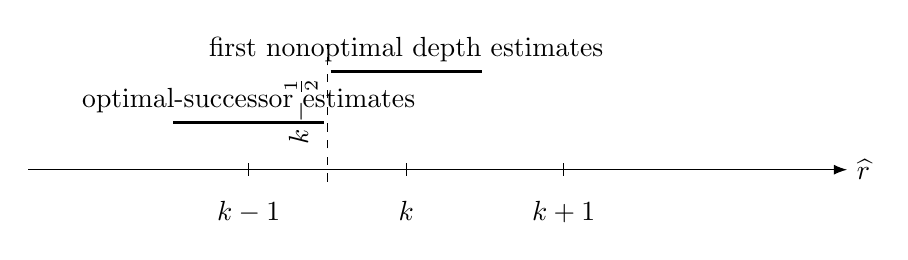
\begin{tikzpicture}[x=2.0cm,y=1cm,>=Latex]
\draw[->] (-0.4,0)--(4.8,0) node[right] {$\rhat$};
\foreach \x/\lab in {1/{k-1},2/{k},3/{k+1}} {
  \draw (\x,0.08)--(\x,-0.08) node[below=2mm] {$\lab$};
}
\draw[very thick] (0.52,0.6)--(1.48,0.6);
\node[above] at (1,0.6) {optimal-successor estimates};
\draw[very thick] (1.52,1.25)--(2.48,1.25);
\node[above,align=center] at (2,1.25) {first nonoptimal\ depth estimates};
\draw[dashed] (1.5,-0.15)--(1.5,1.6);
\node[rotate=90,above] at (1.5,0.75) {$k-\tfrac12$};
\end{tikzpicture}
\caption{With strict error below $1/2$, estimates for depth $k-1$ lie strictly below estimates for depth $k$ or more. The local ordering cannot flip.}
\label{fig:halfstep}
\end{figure}

\begin{remark}[The guarantee is local]
The theorem does not require globally accurate reconstruction of $\rstar$ on every state in $\Basin$. It is sufficient that the estimate preserve the relevant ordering among immediate candidate successors at the states actually visited. This is why local ranking accuracy can matter more operationally than global mean squared error.
\end{remark}

\begin{remark}[Strict inequality matters]
If the error bound is merely $\le1/2$, an optimal successor of true value $k-1$ could be estimated as $k-1/2$ while a nonoptimal successor of true value $k$ could also be estimated as $k-1/2$. A tie-breaking rule could then choose the nonoptimal action. The strict threshold avoids this boundary case.
\end{remark}

\subsection{A ranking formulation}

The numerical approximation is stronger than necessary. What control really requires is the correct local ordering.

\begin{proposition}[Order sufficiency]\label{prop:order}
At a nonterminal state $x$, suppose a score $s$ on candidate successors satisfies
\[
s(y^*)<s(z)
\]
for every optimal successor $y^*$ and every nonoptimal successor $z$. Then every greedy minimizer of $s$ is a shortest-settlement action.
\end{proposition}

\begin{proof}
Under the stated strict separation, no nonoptimal successor can attain the minimum score while an optimal successor exists. Therefore every minimizer is optimal.
\end{proof}

The half-step theorem is a sufficient numerical condition for Proposition \ref{prop:order}. This distinction suggests two experimental targets: regression to $\rstar$ when exact labels are available, and direct pairwise or listwise ranking of candidate actions when only order information is reliable.

\section{Unequal costs and the action-gap theorem}\label{sec:weighted}

Counting every action as one is useful for theory and for expansion-count experiments, but real systems care about wall-clock time, verifier calls, memory, communication, or weighted combinations. The Bellman principle survives, while the integer half-step threshold is replaced by a state-dependent action gap.

\subsection{Positive action costs}

Let
\[
c(x,a)>0
\]
be the cost of taking action $a$ at state $x$. For a finite legal trajectory $x_0,\ldots,x_m$ generated by actions $a_0,\ldots,a_{m-1}$, define total cost
\[
C=\sum_{k=0}^{m-1}c(x_k,a_k).
\]
Define the optimal weighted settlement value
\[
V^*(x)=\inf\{C:\text{a finite legal trajectory from $x$ reaches $\Cset$}\},
\]
with $V^*(x)=+\infty$ when settlement is unreachable.

To obtain an actual minimizing action rather than only an infimum, some attainment condition is required. Finite admissible action sets are sufficient, as are many compactness/lower-semicontinuity conditions familiar from control theory. For a discrete ATP implementation, finiteness of the candidate set considered at each atomic decision is the simplest assumption.

\begin{assumption}[Attained weighted Bellman minimum]\label{ass:attain}
For every nonterminal state under consideration, the quantity
\[
\inf_{a\in\A(x)}\bigl(c(x,a)+V^*(F_a(x))\bigr)
\]
is attained by at least one admissible action.
\end{assumption}

\begin{theorem}[Weighted Bellman optimality]\label{thm:weightedbellman}
Under Assumption \ref{ass:attain}, every nonterminal reachable state satisfies
\[
\boxed{V^*(x)=\min_{a\in\A(x)}\left[c(x,a)+V^*(F_a(x))\right].}
\]
Any minimizing action is an optimal first action for the weighted-cost settlement problem.
\end{theorem}

\begin{proof}
For any first action $a$, every continuation to settlement has total cost at least $c(x,a)+V^*(F_a(x))$. Taking the infimum over all settling trajectories gives
\[
V^*(x)\ge \inf_a\left[c(x,a)+V^*(F_a(x))\right].
\]
Conversely, for any $\varepsilon>0$ and any action $a$, there exists a continuation from $F_a(x)$ with cost at most $V^*(F_a(x))+\varepsilon$ whenever the successor value is finite. Hence
\[
V^*(x)\le c(x,a)+V^*(F_a(x))+\varepsilon.
\]
Taking the infimum over $a$ and then $\varepsilon\downarrow0$ yields the reverse inequality. Assumption \ref{ass:attain} converts the infimum to a minimum. A minimizing first action followed by arbitrarily close-to-optimal continuations achieves the optimal Bellman value; when optimal continuations are attained, concatenation gives an optimal trajectory.
\end{proof}

Define the optimal state-action value
\[
\Qstar(x,a)=c(x,a)+V^*(F_a(x)).
\]
Let
\[
V^*(x)=\min_a\Qstar(x,a).
\]

\begin{definition}[Action gap]
If there is at least one nonoptimal admissible action, define
\[
\Gamma(x)=\inf_{a:\Qstar(x,a)>V^*(x)}\bigl(\Qstar(x,a)-V^*(x)\bigr).
\]
If every admissible action is optimal, set $\Gamma(x)=+\infty$.
\end{definition}

\begin{theorem}[Action-gap robustness theorem]\label{thm:gap}
Suppose $\Gamma(x)>0$ and an estimated state-action value $\widehat Q$ satisfies
\[
|\widehat Q(x,a)-\Qstar(x,a)|<\frac{\Gamma(x)}{2}
\]
for every candidate action $a$. Then every minimizer of $\widehat Q(x,a)$ is truly optimal.
\end{theorem}

\begin{proof}
Let $a^*$ be optimal and $b$ nonoptimal. Then
\[
\Qstar(x,b)-\Qstar(x,a^*)\ge\Gamma(x).
\]
Therefore
\[
\widehat Q(x,a^*)<\Qstar(x,a^*)+\frac{\Gamma(x)}2
\]
and
\[
\widehat Q(x,b)>\Qstar(x,b)-\frac{\Gamma(x)}2
\ge \Qstar(x,a^*)+\frac{\Gamma(x)}2.
\]
Hence every optimal action is estimated below every nonoptimal action. A minimizer of $\widehat Q$ must be optimal.
\end{proof}

In the unit-cost setting, $\Qstar(x,a)=1+\rstar(F_a(x))$, and the gap between an optimal successor of depth $k-1$ and a nonoptimal successor of depth at least $k$ is at least $1$. Theorem \ref{thm:halfstep} is therefore the unit-spaced special case of Theorem \ref{thm:gap}.

\section{Multiple settlement channels and policy meaning}\label{sec:channels}

The abstract terminal set $\Cset$ hides an important feature of AMLDs: there can be several logically different ways to settle the same target. The shortest-settlement theorem remains simple, but the interpretation of ``optimal'' depends on what terminal outcomes and costs the experiment declares.

\subsection{P/R/I/C as terminal subsets}

Let $c$ be a target relative to a fixed formal environment. Write
\[
\Cset_P,\quad \Cset_R,\quad \Cset_I,\quad \Cset_C
\]
for accepted terminal states containing, respectively, a proof of $c$, a proof of $\neg c$, an accepted independence metacertificate of the declared kind, or an inconsistency certificate for the declared base. Then
\[
\Cset=\Cset_P\cup\Cset_R\cup\Cset_I\cup\Cset_C.
\]
Proposition \ref{prop:union} immediately yields
\[
\rstar(x)=\min\{r_P^*(x),r_R^*(x),r_I^*(x),r_C^*(x)\},
\]
where $r_j^*$ is directed unit-cost distance to the corresponding terminal subset, with $+\infty$ for an unreachable channel.

This identity should not be confused with a statement that all outcomes are logically interchangeable. They are interchangeable only as terminal events for the particular objective ``first accepted settlement certificate.'' If the architecture gives contradiction certificates priority, or if it distinguishes a proof from an independence result by utility, then the terminal-cost model must encode that distinction.

\begin{example}[Contradiction-dominant settlement]
Suppose the declared semantics require that an accepted contradiction certificate dominate every other status because an inconsistent base invalidates the intended interpretation of proof and refutation. One can model this by a lexicographic objective: first minimize whether a reachable contradiction is left undetected under the declared audit protocol, then minimize ordinary settlement cost. Alternatively, one can separate a consistency-audit phase from the P/R/I race. What one should not do is silently use the unit-cost union objective and later describe its minimizer as optimal for a different priority rule.
\end{example}

\subsection{Fairness and optimality are different constraints}

A baseline AMLD may require fair scheduling so that complete or semicomplete channels retain liveness guarantees. A purely greedy estimated controller may starve a channel whose current estimated value is poor. The optimality theorem itself is agnostic: it assumes the set of admissible actions $\A(x)$ has already been declared.

There are therefore two clean ways to combine fairness with shortest-settlement control.

First, put fairness state into $x$ and remove actions from $\A(x)$ when the fairness rule requires another channel to receive service. The Bellman theorem then computes the optimum \emph{subject to fairness}. Second, retain all actions but assign costs or penalties that encode the fairness constraint. In either case, the theorem optimizes the problem actually specified.

\begin{remark}[Failure is control information, not a certificate]
A high estimated settlement distance on the P route can rationally shift resources toward R or I. It does not prove that P is impossible. Likewise, prolonged failure may be predictive state information without being a metatheorem. This separation between adaptive control and certificate semantics is a central discipline of the broader AMLD framework \cite{AMLD2,VSS}.
\end{remark}

\section{BANK state and the meaning of distance}\label{sec:bank}

The complete state must include verified memory because the value of a proof-search state depends on what has already been certified. Two logically equivalent axiom bases can have very different operational distances to settlement when one BANK has materialized useful intermediate lemmas and the other has not.

\subsection{A lemma can move the state without changing truth}

Let $x$ contain verified BANK $B$. Suppose $L$ is derivable from the fixed base and a checker accepts a certificate for $L$, producing a state denoted $x\oplus L$. Logically, adding a theorem already derivable from the base need not strengthen the consequence relation. Operationally, it can shorten future search.

\begin{definition}[Marginal settlement value of a verified lemma]
In the unit-cost model define
\[
\Delta_L(x)=\rstar(x)-\rstar(x\oplus L),
\]
whenever both values are finite.
\end{definition}

This is the same operational idea used in the broader BANK-control treatment \cite{VSS}: the point of a reusable lemma is not merely that it is true, but that its verified availability can alter the future geometry of search.

\begin{proposition}[Nonnegative lemma value under free monotone reuse]\label{prop:lemmavalue}
Assume that depositing $L$ incurs no cost in the comparison and that every action sequence available from $x$ remains available from $x\oplus L$. Then
\[
\Delta_L(x)\ge0.
\]
\end{proposition}

\begin{proof}
Every settlement trajectory available from $x$ is also available from $x\oplus L$ by hypothesis. Therefore the minimum settlement length from $x\oplus L$ cannot exceed the minimum from $x$:
\[
\rstar(x\oplus L)\le\rstar(x).
\]
Subtracting gives $\Delta_L(x)\ge0$.
\end{proof}

The hypotheses matter. Real indexing, memory, verification, and search branching can impose overhead, so the practical value of materializing a lemma can be negative under a wall-clock or memory cost model. Weighted value functions in Section \ref{sec:weighted} are the proper place to represent those costs.

\subsection{State sufficiency and learned representations}

The one-dimensional coordinate $\rstar$ always exists on the reachable unit-cost basin. That does not mean the controller can compute it from whatever features happen to be visible.

Let
\[
s:\Basin\to\mathcal S
\]
be a state representation available to a controller. It could contain BANK fingerprints, counts of open goals, verifier outcomes, branch depths, resource counters, selected reflective facts, or a learned embedding.

\begin{definition}[Settlement-sufficient representation]
The representation $s$ is \emph{settlement-sufficient} on a domain $D\subseteq\Basin$ if there exists a function $g$ such that
\[
\rstar(x)=g(s(x))
\]
for every $x\in D$.
\end{definition}

\begin{proposition}[Exact control from a sufficient representation]\label{prop:sufficient}
If $s$ is settlement-sufficient and $g$ is known exactly, then the controller
\[
\pi_s(x)\in\argmin_{a\in\A(x)}g(s(F_a(x)))
\]
selects a shortest-settlement action at every nonterminal $x\in D$ whose relevant successors also lie in $D$.
\end{proposition}

\begin{proof}
Settlement sufficiency gives $g(s(F_a(x)))=\rstar(F_a(x))$ for every candidate successor. The stated minimization is therefore exactly the optimal-action rule of Theorem \ref{thm:bellman}.
\end{proof}

\begin{corollary}[Approximate control from a sufficient representation]
If $s$ is settlement-sufficient with $\rstar=g\circ s$ and an estimator $\widehat g$ satisfies
\[
|\widehat g(s(y))-g(s(y))|<\frac12
\]
for every immediate successor $y$ compared by the controller, then greedy minimization of $\widehat g\circ s$ selects a shortest-settlement action in the unit-cost model.
\end{corollary}

\begin{proof}
Apply Theorem \ref{thm:halfstep} to $\rhat=\widehat g\circ s$.
\end{proof}

This result clarifies what a low-dimensional learned representation must accomplish. It need not reconstruct the theorem prover. It must preserve enough information to rank the next actions by their effect on optimal remaining settlement cost.

\begin{storybox}[A map that omits the color of the buildings]
A road map can be excellent for navigation while saying nothing about the color of the houses. Likewise, a settlement representation can be excellent for control while discarding most of the internal details of an AMLD. The question is not whether the representation is a complete portrait of the machine. The question is whether the discarded information changes $\rstar$ or, more modestly, changes the ordering of the immediate actions.
\end{storybox}

\section{What the optimality theorem does not compute}\label{sec:limits}

The phrase ``the optimal strategy is known'' can be misunderstood. The theorem identifies the strategy in terms of the exact value function:
\[
\pi^*(x)\in\argmin_a\rstar(F_a(x)).
\]
That is a complete mathematical characterization. It is not a promise that $\rstar$ is cheaply computable on arbitrary formal systems.

This distinction is standard in optimization. A variational characterization can be exact while evaluating the optimum remains hard. In theorem search the limitation is sharper because sufficiently expressive derivability problems are undecidable.

\subsection{An exact total oracle would decide derivability}

We formulate the obstruction at the level needed here.

\begin{assumption}[Theorem-search encoding]\label{ass:encoding}
Let $T$ be an effectively presented formal theory with undecidable theorem set. For each sentence $\varphi$, suppose one can effectively construct an initial AMLD state $x_\varphi$ such that
\[
x_\varphi\in\Basin\quad\Longleftrightarrow\quad T\vdash\varphi,
\]
and settlement in this restricted encoding means acceptance of a finite $T$-proof of $\varphi$.
\end{assumption}

Such encodings are routine for ordinary proof enumeration in recursively axiomatized theories with decidable proof checking; practical ATP texts describe this basic semidecision setting \cite{Harrison,Metamath}.

\begin{theorem}[No total computable exact settlement-distance oracle on an undecidable theorem class]\label{thm:undecidable}
Under Assumption \ref{ass:encoding}, there is no total computable function
\[
R(x_\varphi)\in\N_0\cup\{\infty\}
\]
satisfying
\[
R(x_\varphi)=
\begin{cases}
\rstar(x_\varphi),&x_\varphi\in\Basin,\\
\infty,&x_\varphi\notin\Basin,
\end{cases}
\]
for every sentence $\varphi$.
\end{theorem}

\begin{proof}
Suppose such a total computable $R$ existed. Given any sentence $\varphi$, effectively construct $x_\varphi$ and compute $R(x_\varphi)$. By the specification of $R$ and Assumption \ref{ass:encoding},
\[
T\vdash\varphi\quad\Longleftrightarrow\quad R(x_\varphi)<\infty.
\]
Thus theoremhood in $T$ would be decidable, contradicting the assumed undecidability of the theorem set.
\end{proof}

\begin{corollary}[Existence is not effective universality]
The exact settlement coordinate $\Phi(x)=\rstar(x)$ can exist mathematically on the reachable basin even though no total computable procedure can return the exact finite value on every provable target and $\infty$ on every unprovable target for an undecidable theorem class.
\end{corollary}

This is the key boundary. The one-dimensional quotient theorem is not a hidden solution of undecidability. It says that if one knew the optimal remaining distance, the optimal control law would be immediate. The scientific problem is to estimate useful local order information without pretending to possess an impossible universal oracle.

\subsection{Exact labels are available on finite controlled benchmarks}

The limitation does not prevent exact value labels on finite search graphs. If an experiment freezes a finite directed state graph and a terminal set, reverse breadth-first search computes exact unit-cost settlement depths for every state that can reach settlement.

\begin{proposition}[Finite reverse-distance computation]\label{prop:reversebfs}
Let $G=(V,E)$ be a finite directed graph of AMLD states and legal unit-cost transitions, with terminal set $C\subseteq V$. Then exact values
\[
\rstar(v)=\min_{s\in C}\delta(v,s)
\]
for all reachable $v$ can be computed by breadth-first search on the reversed graph beginning from all vertices in $C$.
\end{proposition}

\begin{proof}
A directed path of length $m$ from $v$ to $C$ in $G$ corresponds exactly to a directed path of length $m$ from $C$ to $v$ in the edge-reversed graph. Multi-source breadth-first search returns the shortest such path length in a finite unit-cost graph.
\end{proof}

This supplies a principled training and evaluation regime: solve or enumerate manageable sealed graphs, compute exact $\rstar$ retrospectively, train a compass on permitted states, and evaluate action ordering on withheld states or targets. The theorem does not eliminate experimentation; it tells the experiment exactly what quantity to measure.

\section{From theorem to controller}\label{sec:controller}

The mathematical strategy is now fully specified. The engineering problem is to approximate it without introducing a new source of proof authority.

\subsection{Verifier sovereignty}

The controller may be uncertain. The verifier should not be. A settlement-distance model can rank candidate actions, allocate resources, or decide which branch to expand next. It should not change whether a fixed proof certificate is valid.

This yields a clean architectural separation:
\[
\text{state observation}\longrightarrow\text{candidate actions}\longrightarrow\text{distance estimates}
\longrightarrow\text{control choice}\longrightarrow\text{ordinary verifier}.
\]
The learned model chooses what to try. The checker decides what has been proved.

\begin{figure}[ht]
\centering
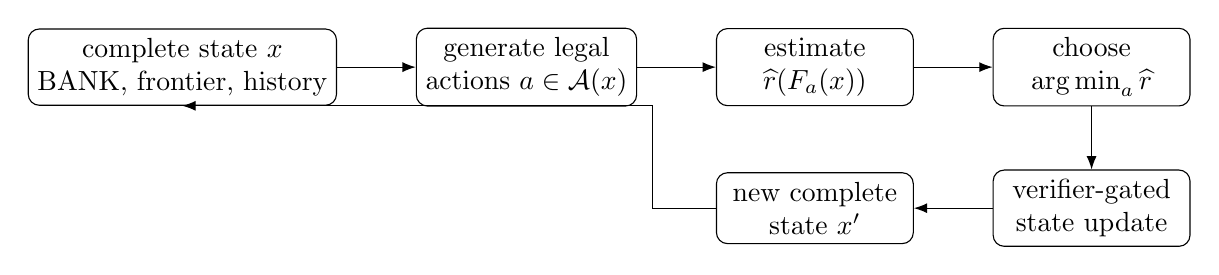
\begin{tikzpicture}[>=Latex,node distance=8mm and 10mm,
 box/.style={draw,rounded corners,align=center,minimum height=9mm,minimum width=25mm}]
\node[box] (state) {complete state $x$\\BANK, frontier, history};
\node[box,right=of state] (cand) {generate legal\\actions $a\in\A(x)$};
\node[box,right=of cand] (eval) {estimate\\$\rhat(F_a(x))$};
\node[box,right=of eval] (pick) {choose\\$\argmin_a\rhat$};
\node[box,below=of pick] (verify) {verifier-gated\\state update};
\node[box,left=of verify] (new) {new complete\\state $x'$};
\draw[->] (state)--(cand); \draw[->] (cand)--(eval); \draw[->] (eval)--(pick);
\draw[->] (pick)--(verify); \draw[->] (verify)--(new);
\draw[->] (new.west) -- ++(-8mm,0) |- (state.south);
\end{tikzpicture}
\caption{A settlement compass changes search control, not certificate semantics. Every accepted mathematical deposit still passes through the declared verifier.}
\label{fig:controller}
\end{figure}

\subsection{Compass-first best-first search}

A practical search node can be assigned a priority resembling
\[
\widehat f(x)=g(x)+\rhat(x),
\]
where $g(x)$ is cost already spent along the represented branch and $\rhat(x)$ estimates remaining settlement cost. The exact form depends on whether the search frontier represents mutually exclusive trajectories, reusable shared BANK state, or a more complex multi-agent federation. The central design principle is invariant: estimated distance-to-settlement should be treated as a control objective rather than as an ornamental feature added after heuristic ranking.

The following pseudocode states the minimal local controller.

\begin{tcolorbox}[colback=softgray,colframe=linegray,title={Compass controller: unit-cost local decision}]
\begin{verbatim}
INPUT: complete state x
IF x is terminal: HALT with verified settlement
GENERATE admissible actions A(x)
FOR each a in A(x):
    y[a] <- verified/legal successor description F_a(x)
    score[a] <- r_hat(y[a])
CHOOSE a_hat minimizing score[a]
EXECUTE a_hat
VERIFY every proposed mathematical deposit by the ordinary checker
RETURN the resulting complete state
\end{verbatim}
\end{tcolorbox}

Exploration can be retained as a safety mechanism when $\rhat$ is imperfect. One can reserve a fraction of the action budget for lower-ranked but legal alternatives, maintain a fair fallback schedule, or use an ensemble of compasses. Such additions may improve empirical robustness, but they change the realized policy away from the exact greedy law. That is acceptable so long as the comparison is explicit.

\subsection{What should be learned?}

There are at least four increasingly ambitious targets.

\begin{enumerate}
\item \textbf{Binary local preference:} given two successors, predict which has smaller $\rstar$.
\item \textbf{Listwise action ranking:} order all current successors by $\rstar$.
\item \textbf{Scalar regression:} estimate $\rstar(y)$ itself.
\item \textbf{Weighted state-action value:} estimate $\Qstar(x,a)$ under a realistic cost function.
\end{enumerate}

The theorems in this paper make clear that exact scalar regression is not logically necessary. Correct local ordering suffices. The scalar target is nevertheless attractive because it can be calibrated, compared across states, inserted into Bellman residuals, and interpreted geometrically.

\section{A motivating Halo(0) application}\label{sec:halo}

A current motivating application is the formal search for the Halo(0) target in a Metamath-based environment. The details of that conjecture are not needed for any theorem in this paper. What matters here is the experimental pattern: the target proof is withheld, a search engine generates candidate proof states, and success is recognized only when an emitted certificate is accepted by an independent Metamath verifier.

The settlement theory recommends a change in what the search engine tries to predict. A generic structural heuristic may prefer fewer hypotheses, smaller syntax trees, novel assertion labels, or diverse branches. Those signals can be useful, but none is by definition the objective. The objective is
\[
\rstar(x)=\text{minimum remaining cost to a verified terminal certificate}.
\]
A settlement-compass variant therefore treats a blind surrogate $\rhat$ of successor settlement distance as the primary control signal while leaving verification untouched.

\begin{caution}[No theorem about the quality of a particular surrogate]
Theorem \ref{thm:halfstep} states what follows \emph{if} $\rhat$ is accurate to less than $1/2$ on the compared unit-cost successors. It does not prove that a given feature formula, neural model, or heuristic score satisfies that condition on Halo(0) or on any other difficult target. That is an empirical question.
\end{caution}

This distinction is scientifically useful. It converts an imprecise claim such as ``the heuristic seems more proof-directed'' into measurable questions:
\begin{itemize}
\item How often does $\rhat$ rank an optimal successor above every nonoptimal successor on finite held-out graphs where $\rstar$ is known?
\item What fraction of comparisons satisfy the half-step condition?
\item Does compass guidance reduce verifier calls or wall-clock time to settlement under fixed resources?
\item Does the improvement survive leakage-resistant target withholding and negative controls?
\end{itemize}

The open-target run comes last, not first. On an open or extremely difficult target, failure to emit a certificate remains merely an unsuccessful run under finite resources.

\section{A theorem-driven experimental program}\label{sec:experiments}

A good experiment should test the mathematical mechanism rather than merely compare two opaque programs. The settlement theorems suggest a staged design.

\subsection{Stage I: exact finite geometry}

Construct finite or finitely truncated proof-search graphs for solved targets. Hide final certificates from the learning procedure but retain them for retrospective labeling. Compute exact $\rstar$ by reverse breadth-first search. Record, for each nonterminal state:
\begin{itemize}
\item the exact value $\rstar(x)$;
\item the set $\A^*(x)$ of optimal actions;
\item the gap between optimal and nonoptimal successor values;
\item state features available to the compass;
\item whether BANK additions alter future depth.
\end{itemize}

Train on one set of targets and evaluate on withheld targets. The primary local metric is optimal-action recovery, not merely scalar error.

\subsection{Stage II: closed-loop sealed settlement}

Deploy the learned compass in complete searches. Freeze the formal environment, target set, verifier, action generator, resource budget, random seeds, and fallback policy before evaluation. Compare at least:
\begin{enumerate}
\item an unguided or standard best-first baseline;
\item the existing structural heuristic;
\item the settlement compass;
\item a randomized-ranking negative control preserving candidate coverage.
\end{enumerate}

The primary endpoint is verified settlement under fixed resources. Secondary endpoints include expansions, verifier calls, wall-clock time, peak memory, and the fraction of encountered states where retrospective analysis shows the chosen action was truly optimal.

\subsection{Stage III: difficult and unknown targets}

Only after the mechanism transfers to sealed targets should it be tested on genuinely difficult mathematics. The outcome categories must remain conservative:
\begin{center}
verified certificate, verified refutation, accepted declared metacertificate, accepted inconsistency certificate, or UNKNOWN under the resource bound.
\end{center}
No distance estimate, confidence score, or repeated failure is itself a settlement certificate.

\subsection{Ablations that matter}

The most informative ablations are those suggested by the theory. Remove BANK features while keeping syntax. Remove history while keeping BANK. Replace scalar $\rhat$ with pairwise ranking. Remove exploration. Keep the compass but randomize its outputs. Train on raw proof depth rather than settlement distance. These tests ask which state information is actually sufficient for the local ordering implied by Bellman optimality.

\begin{storybox}[Why a negative result is useful]
Suppose a learned compass predicts exact $\rstar$ poorly but still chooses an optimal action 82\% of the time. That may be operationally valuable because Proposition \ref{prop:order} cares about ordering. Conversely, suppose a model achieves low mean squared error by being excellent on easy states but repeatedly reverses the top two actions near difficult bottlenecks. Its global regression score can look good while its control policy is poor. The theorem tells us which failure matters.
\end{storybox}

\section{Common misreadings and their corrections}\label{sec:misreadings}

Because the central result is simple once written down, it is easy to accidentally claim more than it proves. This section records the main boundaries explicitly.

\subsection{``The full state space is one-dimensional''}

False in general. The theorem says that the quotient by equal optimal settlement depth is one-dimensional. The complete AMLD state can contain arbitrarily rich verified and operational information. The map $\Phi(x)=\rstar(x)$ is usually many-to-one.

\subsection{``Euclidean distance reproduces all proof-search distances''}

False in general. Legal search is directed and often irreversible. Proposition \ref{prop:noeuclid} rules out exact representation of an asymmetric directed distance by an ordinary symmetric Euclidean metric.

\subsection{``Knowing the theorem gives an efficient solver''}

False. The theorem gives the optimal feedback law in terms of $\rstar$. Theorem \ref{thm:undecidable} shows that a total exact computable oracle for finite-versus-infinite settlement distance cannot exist on a theorem class whose derivability relation is undecidable under the stated encoding.

\subsection{``A gradient can be taken directly in the raw AMLD state''}

Not without additional structure. $\X$ is an abstract controlled state space, not automatically a differentiable manifold or vector space. The gradient statement in this paper is exact on the one-dimensional settlement quotient. Learned embeddings of the raw state can support additional differential approximations, but those are modeling choices rather than consequences of the theorem.

\subsection{``The shortest proof is always the right practical objective''}

Not necessarily. Unit action cost minimizes the number of control steps. A shorter proof trajectory can take more wall-clock time if its steps are expensive. Section \ref{sec:weighted} replaces step count by declared positive costs. The optimal policy is always relative to an objective.

\subsection{``Independence can be inferred from long failure''}

No. Failure history can influence a controller's ranking of future actions, but an independence outcome requires the declared metacertificate. The settlement set is defined by accepted terminal certificates, not by confidence or elapsed time.

\section{A compact theorem map}\label{sec:map}

\begin{longtable}{p{0.25\textwidth}p{0.16\textwidth}p{0.51\textwidth}}
\toprule
\textbf{Result} & \textbf{Type} & \textbf{Meaning}\\
\midrule
\endhead
Directed graph distance & Proposition \ref{prop:directedmetric} & Legal search generates a directed extended distance satisfying identity and triangle inequality but not necessarily symmetry.\\
\addlinespace
Settlement zero set & Proposition \ref{prop:zeroset} & Distance zero is exactly terminal settlement.\\
\addlinespace
Distance-time identity & Theorem \ref{thm:distanceequals} & Directed distance to the terminal set equals optimal remaining unit-cost settlement time.\\
\addlinespace
Bellman optimality & Theorem \ref{thm:bellman} & The optimal first move minimizes successor settlement distance.\\
\addlinespace
Optimal feedback & Corollary \ref{cor:policy} & Repeatedly choosing a minimizing successor settles in exactly $\rstar(x_0)$ steps.\\
\addlinespace
Geodesic criterion & Proposition \ref{prop:geodesic} & A path is shortest exactly when $\rstar$ drops by one at every step.\\
\addlinespace
One-dimensional quotient & Theorem \ref{thm:quotient} & Equal-depth states quotient to an initial segment of $\N_0\subset\R$ isometrically.\\
\addlinespace
Optimal shift conjugacy & Theorem \ref{thm:conjugacy} & Quotient optimal dynamics are exactly $k\mapsto\max(k-1,0)$.\\
\addlinespace
Discrete gradient & Theorem \ref{thm:gradient} & Optimal actions are exactly the legal one-unit descent directions in the settlement coordinate.\\
\addlinespace
Half-step compass & Theorem \ref{thm:halfstep} & Successor error $<1/2$ preserves shortest-action choice in the unit-cost model.\\
\addlinespace
Action-gap robustness & Theorem \ref{thm:gap} & Weighted value error below half the true action gap preserves optimal control.\\
\addlinespace
Undecidability boundary & Theorem \ref{thm:undecidable} & Exact settlement geometry does not create a total computable theorem-decider on undecidable classes.\\
\bottomrule
\end{longtable}

\section{Conclusion}

The shortest-settlement problem has a precise solution.

Start with a complete AMLD state $x$, its legal actions $\A(x)$, deterministic successor maps $F_a$, and a verifier-defined terminal settlement set $\Cset$. Legal actions generate an intrinsic directed graph geometry. In the unit-cost model, the distance from $x$ to $\Cset$ is exactly the optimal remaining settlement time:
\[
\dset(x)=\rstar(x).
\]
The Bellman equation then gives
\[
\rstar(x)=1+\min_a\rstar(F_a(x)),
\]
so the optimal strategy is
\[
\boxed{\pi^*(x)\in\argmin_a\rstar(F_a(x)).}
\]
Repeated optimal choices reduce $\rstar$ by exactly one until the verifier-defined terminal set is reached.

The geometry can be compressed without approximation. States of equal $\rstar$ form equivalence classes, and the resulting settlement quotient is isometric to an initial segment of the nonnegative integers on the real line. Under any optimal policy, the quotient dynamics are conjugate to
\[
k\longmapsto\max(k-1,0).
\]
Thus the complete machine need not be Euclidean, but its optimal settlement dynamics possess an exact one-dimensional Euclidean factor. In that factor, distance to settlement is ordinary distance to zero and the optimal move is the discrete negative-gradient step. Reversing sign gives the Abel coordinate $h^*=-\rstar$, which advances by one under optimal motion.

The central practical difficulty is therefore no longer conceptual. It is estimation. Exact $\rstar$ can be unavailable or noncomputable as a total oracle on sufficiently expressive theorem classes. But a controller does not need metaphysical access to the whole proof landscape. In the unit-cost setting, a local estimate within strict half-step error on the candidate successors recovers a true shortest-settlement action. More generally, prediction error below half the action gap preserves weighted optimality.

This changes the research question from ``can proof search be given a geometry?'' to a sharper one:
\begin{center}
\emph{Can a verifier-neutral model learn enough of the settlement quotient to preserve the local action ordering on unseen search states?}
\end{center}
That question is mathematical, computational, and experimentally falsifiable. The verifier still has the last word.

\appendix

\section{A fully worked finite example}\label{app:example}

This appendix computes the entire settlement geometry of a small directed search graph. The example is intentionally elementary because its purpose is to make every object in the main theorem visible at once.

Consider states
\[
\{x_0,x_1,x_2,x_3,x_4,x_5,s_P,s_R\}
\]
with terminal set $\Cset=\{s_P,s_R\}$. The legal transitions are
\[
\begin{aligned}
x_0&\to x_1,\quad x_0\to x_2,\quad x_0\to x_3,\\
x_1&\to x_4,\quad x_1\to x_5,\\
x_2&\to x_5,\\
x_3&\to x_2,\\
x_4&\to s_P,\\
x_5&\to x_4,\quad x_5\to s_R.
\end{aligned}
\]
Every edge has unit cost.

Working backward from the terminal set gives
\[
\rstar(s_P)=\rstar(s_R)=0.
\]
State $x_4$ has a direct transition to $s_P$, so $\rstar(x_4)=1$. State $x_5$ has a direct transition to $s_R$, so $\rstar(x_5)=1$ even though it also has a longer route through $x_4$. Then
\[
\rstar(x_1)=1+\min\{\rstar(x_4),\rstar(x_5)\}=2,
\]
and
\[
\rstar(x_2)=1+\rstar(x_5)=2.
\]
Next,
\[
\rstar(x_3)=1+\rstar(x_2)=3.
\]
Finally,
\[
\rstar(x_0)=1+\min\{2,2,3\}=3.
\]

Thus the quotient classes are
\[
\begin{aligned}
L_0&=\{s_P,s_R\},\\
L_1&=\{x_4,x_5\},\\
L_2&=\{x_1,x_2\},\\
L_3&=\{x_0,x_3\}.
\end{aligned}
\]
Notice that $x_0$ and $x_3$ have equal optimal depth despite having different positions and outgoing actions in the complete graph.

At $x_0$, the actions leading to $x_1$ and $x_2$ are optimal because both successors have value $2$. The action leading to $x_3$ is nonoptimal because its successor has value $3$. If an estimate $\rhat$ satisfies strict half-step error, then
\[
\rhat(x_1),\rhat(x_2)\in(1.5,2.5)
\]
while
\[
\rhat(x_3)\in(2.5,3.5).
\]
Therefore $x_3$ cannot be ranked ahead of both optimal successors.

The quotient dynamics under any optimal selector are simply
\[
3\to2\to1\to0.
\]
The complete state graph contains branching, multiple terminals, and a nonoptimal detour. The settlement quotient contains only optimal depth. This is exactly what the main theorem asserts in general.

\section{Proof checklist for implementations}\label{app:checklist}

When translating the theorems into software or a formal proof assistant, the following items should be checked explicitly.

\begin{enumerate}
\item \textbf{State completeness.} Every variable that can change successor generation or action legality is represented in $x$ or frozen externally.
\item \textbf{Terminal semantics.} Membership in $\Cset$ is tied to an accepted declared certificate, not to a heuristic confidence value.
\item \textbf{Action legality.} $\A(x)$ contains only declared control operations. Learned guidance ranks actions but does not invent unchecked inference rules.
\item \textbf{Cost model.} Unit cost, verifier-call cost, wall-clock cost, or another objective is stated before ``optimal'' is used.
\item \textbf{Reachability domain.} Exact finite $\rstar$ claims are restricted to the settlement basin or explicitly use $+\infty$ outside it.
\item \textbf{Bellman target.} If training labels are called settlement distance, verify that they correspond to the same transition graph and cost model used at evaluation time.
\item \textbf{No leakage.} A withheld target's reference proof is not used to train, rank, engineer theorem-specific features, or tune hyperparameters.
\item \textbf{Independent verification.} A discovered certificate is checked by a verifier whose acceptance semantics do not depend on the compass score.
\item \textbf{Unknown remains unknown.} Timeout or search failure is not promoted to refutation or independence.
\item \textbf{Reproducibility.} Record environment version, target, seed, budget, action generator, model version, and verifier version.
\end{enumerate}

\section{Notation reference}\label{app:notation}

\begin{longtable}{p{0.20\textwidth}p{0.70\textwidth}}
\toprule
\textbf{Symbol} & \textbf{Meaning}\\
\midrule
\endhead
$\X$ & Complete AMLD state space.\\
$\Cset$ & Verifier-defined terminal settlement set.\\
$\Basin$ & States from which some finite legal trajectory reaches $\Cset$.\\
$\A(x)$ & Admissible control actions at state $x$.\\
$F_a(x)$ & Successor state after action $a$.\\
$\delta(x,y)$ & Directed unit-cost legal path distance from $x$ to $y$.\\
$\dset(x)$ & Directed distance from $x$ to the settlement set.\\
$\rstar(x)$ & Optimal remaining number of unit-cost steps to settlement.\\
$\A^*(x)$ & Set of shortest-settlement actions at $x$.\\
$\Phi(x)$ & Settlement coordinate $\rstar(x)$.\\
$h^*(x)$ & Abel coordinate $-\rstar(x)$.\\
$\rhat(x)$ & Estimated settlement distance.\\
$V^*(x)$ & Optimal remaining weighted settlement cost.\\
$\Qstar(x,a)$ & Weighted optimal state-action value.\\
$\Gamma(x)$ & Gap between the optimal action value and the best strictly nonoptimal value.\\
$\Pi_{\Cset}(x)$ & Set of nearest terminal settlement states.\\
\bottomrule
\end{longtable}

\section*{AI Integrity Statement}
\addcontentsline{toc}{section}{AI Integrity Statement}
AI assistance was used in the preparation of exposition, organization, typesetting, and the testing and refinement of proof formulations in this Version 1.0 manuscript. The author supplied the research program, the AMLD settlement setting, the motivating geometric question, and the direction of the optimality investigation. Mathematical statements labeled theorem, proposition, lemma, or corollary were written with explicit hypotheses and checked for internal consistency during preparation, but they remain appropriate subjects for independent scholarly review and, where feasible, formal verification. No open conjecture is claimed settled in this article without an independently checkable certificate.

\section*{Author Note}
\addcontentsline{toc}{section}{Author Note}
Brian Tenneson earned an M.S. in Applied Data Science from Bay Path University in 2025, an M.A. in Mathematics from San Francisco State University in 2001, and a B.A. in Mathematics from the University of California, Berkeley, in 1998. His current research interests include automated theorem proving, verifier-gated conjecture settlement, machine-guided proof search, formal systems, and the geometry and control of mathematical discovery. He is currently unaffiliated. Contact: \href{mailto:btenneson2301@baypath.edu}{btenneson2301@baypath.edu}. Essays and project notes: \url{https://brian2301.substack.com}.

\begin{thebibliography}{99}

\bibitem{VSS}
Brian Tenneson.
\newblock \emph{Verified Settlement Search: BANKs, Formal Self-Description, Controlled IFS Dynamics, Abel--Bellman Navigation, and a Return to Conjectures}.
\newblock Version 1.4, August 22, 2026.

\bibitem{Checks}
Brian Tenneson.
\newblock \emph{What Checks the Proof? A Textbook Introduction to Automated Mathematical Logic Deciders: BANK, FUTUREBANK, Imagination, Compass, Verification, Controlled Creativity, and Formalized Self-Awareness}.
\newblock Textbook Version 6.80, August 22, 2026.

\bibitem{DATA3}
Brian Tenneson.
\newblock \emph{DATA 3.0 AMLD IFS Semigroup Architecture}.
\newblock Working technical manuscript, August 2026.

\bibitem{Compass}
\newblock \emph{Proof Compass Theory: Learnability, Shrinkage, and Control}.
\newblock Technical report prepared for Brian Tenneson, August 15, 2026.
\newblock Public project pointer: \url{https://github.com/btenneson/pub/tree/main/cs.LO_Logic_in_Computer_Science/Proof_Compass_Theory}.

\bibitem{AMLDControl}
Brian Tenneson.
\newblock \emph{AMLD Compass--Control Integration: Value Functions, Lyapunov and Abel Coordinates, Theorem-Shell Control, and Proof-Ocean Navigation}.
\newblock August 14, 2026.

\bibitem{AMLD2}
Brian Tenneson.
\newblock \emph{Automatic Metalogical Deciders, Part Two: Conjectures Revealed}.
\newblock Revised edition, August 12, 2026.

\bibitem{Bellman}
Richard Bellman.
\newblock \emph{Dynamic Programming}.
\newblock Princeton University Press, 1957.

\bibitem{Hutchinson}
John E. Hutchinson.
\newblock Fractals and self-similarity.
\newblock \emph{Indiana University Mathematics Journal}, 30(5):713--747, 1981.
\newblock DOI: 10.1512/iumj.1981.30.30055.

\bibitem{Harrison}
John Harrison.
\newblock \emph{Handbook of Practical Logic and Automated Reasoning}.
\newblock Cambridge University Press, 2009.

\bibitem{Metamath}
Norman D. Megill and David A. Wheeler.
\newblock \emph{Metamath: A Computer Language for Mathematical Proofs}.
\newblock Second edition, 2019.
\newblock \url{https://us.metamath.org/downloads/metamath.pdf}.

\end{thebibliography}

\end{document}
